\begin{figure}[t]
  \center
  \def\layersep{4cm}
  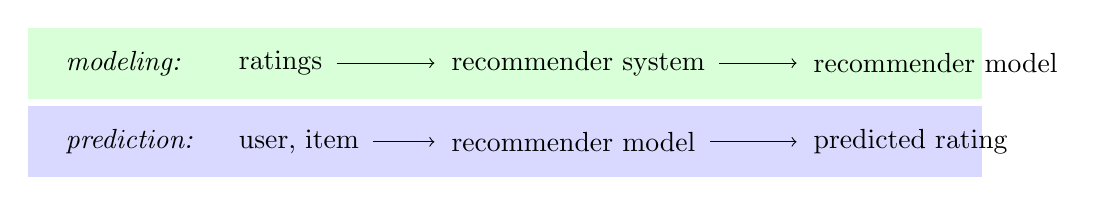
\begin{tikzpicture}[shorten >=1pt,->,draw=black, node distance=\layersep]

    \tikzstyle{every pin edge}=[<-,shorten <=2pt]
    \tikzstyle{rmodel}=[rectangle,fill=green!25,minimum size=20pt,inner sep=5pt]
    \tikzstyle{emodel}=[rectangle,fill=blue!25,minimum size=20pt,inner sep=5pt]
    \tikzstyle{amodel}=[rectangle,fill=red!25,minimum size=20pt,inner sep=5pt]
    \tikzstyle{blank}=[rectangle,right,fill=none,minimum size=20pt,inner sep=5pt]
      
    \fill[green!15] (0,1.1) rectangle (\textwidth,2);
    \fill[blue!15] (0,0.1) rectangle (\textwidth,1);
    
    \node[blank] (I2) at (0.3cm,  0.55) {\emph{prediction:}};
    \node[blank] (I1) at (0.3cm,  1.55)  {\emph{modeling:}};
    
    \node[blank] (I2) at (2.5cm, 0.55) {user, item};
    \node[blank] (I1) at (2.5cm, 1.55) {ratings};
   
    \node[blank] (P2) at (5.2cm, 0.55) {recommender model};
    \node[blank] (P1) at (5.2cm, 1.55) {recommender system};

    \node[blank] (O2) at (9.8cm, 0.55) {predicted rating};
    \node[blank] (O1) at (9.8cm, 1.55) {recommender model};
    
    \path (I1) edge (P1);
    \path (I2) edge (P2);

    \path (P1) edge (O1);
    \path (P2) edge (O2);
       
  \end{tikzpicture}

  \vspace{1em}
  \caption[Simplified Recommender System]{
    A simplified view of recommender systems:
    Ratings of items by users are used to create a \emph{model}.
    This model is then used to predict unknown ratings between users and items.
    Note that many recommender systems work differently,
    as we shall soon see.
  }
  \label{fig:simple-rs}
\end{figure}
